\section{Queuing Model (90 pts)}

% Note that for queuing models it is enough to use the experimental results from the previous sections. It is, however, possible that the numbers you need are not only the ones in the figures we asked for, but also the internal measurements that you have obtained through instrumentation of your middleware.
In this section, we model the system with different queuing models and analyze the similarities and differences between model predictions and actual measurements. Common notations that are used in all subsections include: traffic intensity ($\rho$: \%) mean arrival rate ($\lambda$: ops/sec), service time per job ($s$: ms), mean service rate per server ($\mu$: ops/sec), number of jobs in the system ($n$: ops), number of jobs waiting in the queue ($n_q$: ops), number of jobs receiving service ($n_s$: ops), response time or time in the system ($r$: ms) and waiting time between arrival and service start ($w$: ms).
% It is always assumed that the inter-arrival time distribution and the service time distribution are exponential distributions.

\subsection{M/M/1}

For each worker-thread configuration in Section 4, we model the entire closed system with one M/M/1 queue, and compare the output parameters with actual measurements. As input, the arrival rate $\lambda$ is set to the average throughput measured by memtier clients, instead of the average arrival rate measured by the network thread of the middleware, because when modelling the entire system as a whole, the best-effort estimation of arrival rate should have been done by the load generator. The service rate $\mu$ is set to the maximum memtier-measured throughput that has been observed under the same work-thread configuration, regardless of the number of clients, because this from the observations gives a best lower bound of the real service rate.

Because an M/M/1 queue is too much abstraction for the system, there is no ``correct'' way to map it to our system's actual components. Here we define the waiting/service separation point as the moment a request starts to be served by the memcached server, therefore, $E[s]$ is the middleware-measured memcached service time,
$E[n_q]$ is the average length of the middleware request queue,
$E[r]$ is the memtier-measured response time,
and $E[w]$ is $E[r]-E[s]$. 

\begin{table}[!ht]
\resizebox{\linewidth}{!}{%
\begin{tabular}{l|cc|cc|cc|cc}
\hline
          & \multicolumn{2}{c|}{8 Workers} & \multicolumn{2}{c|}{16 Workers} & \multicolumn{2}{c|}{32 Workers} & \multicolumn{2}{c}{64 Workers} \\ \cline{2-9} 
          & Predicted             & Measured            & Predicted             & Measured             & Predicted             & Measured             & Predicted             & Measured             \\ \hline
$\lambda$ & -                     & 7562.64             & -                     & 9214.13              & -                     & 10842.41             & -                     & 12932.08             \\
$\mu$     & -                     & 7694.54             & -                     & 9604.29              & -                     & 11240.95             & -                     & 13234.23             \\
$\rho$    & 98.29\%               & -                   & 95.94\%               & -                    & 96.45\%               & -                    & 97.72\%               & -                    \\
$E[s]$    & 0.13                  & 1.97                & 0.10                  & 3.08                 & 0.09                  & 5.46                 & 0.08                  & 9.32                 \\
$E[n_q]$  & 56.35                 & 6.21                & 22.66                 & 2.71                 & 26.24                 & 6.51                 & 41.82                 & 16.95                \\
$E[w]$    & 7.45                  & 2.73                & 2.46                  & 2.08                 & 2.42                  & 3.30                 & 3.23                  & 5.09                 \\ 
$E[r]$    & 7.58                  & 4.70                & 2.56                  & 5.16                 & 2.51                  & 8.76                 & 3.31                  & 14.64                \\ \hline
\end{tabular} %
}
\captionsetup{belowskip=0em,aboveskip=4pt}
\caption{\label{tab:mm1}Results of M/M/1 Model}
\end{table}

For each worker-thread configuration, Table~\ref{tab:mm1} is acquired based on the formulae in Box 31.1 from the textbook. Note that the experiments have been repeated for different number of clients. For brevity, only results for the saturation points (as summarized in Section 4.1.1 and 4.2) are listed, namely 36, 48, 96, 192 clients for 8, 16, 32, 64 worker threads respectively. All $\rho$ values are below 100\%, so the system is stable.



Comparing between model predictions and experiment results, we find that a simple M/M/1 model is far from reporting the real life behaviour of the system. (1) The predicted mean service time $E[s]$ is much lower than reality, because M/M/1 cannot model the parallel request processing pattern of the system: the high arrival rate is actually not a result of low service time, but due to the fact that there are multiple workers processing multiple requests at the same time, but with M/M/1 the service time is just the inverse of arrival rate. (2) The predicted mean number of jobs $E[n_q]$ in the queue is much larger than reality, because there are more than one queues in the whole system (as we will show in Section 7.3), but M/M/1 has abstracted everything into one queue, and the length of middleware request queue is only a part of the queue length reported by this model. (3) The predicted mean response time $E[r]$ also has a large discrepancy from the reality, and does not follow the increasing trend of real response time with regard to the number of workers, because the model is not aware of the parallel processing of workers. (4) The mean waiting time in the queue $E[w]$ seems to be a little bit close to reality, but this is just a coincidence made by the choice of client numbers, for other numbers of clients with similar arrival rates, the predicted $E[w]$ will be similar but the measured waiting time could completely change, e.g. due to over-saturation.

Therefore, an M/M/1 model is over-simplified for our system, and indeed it cannot model the characteristics of the entire system satisfactorily.

\subsection{M/M/m}

In order to better model the multi-processing nature of the system, next we build an M/M/m model based on Section 4, where each middleware worker thread is represented as one service, therefore $m=$ the total number of worker threads in two middlewares. The arrival rate $\lambda$ is again set to the average throughput measured by memtier as it is the load generator and provides the best-effort estimation. The service rate $\mu$ of one service is set to the same $\mu$ in M/M/1 but divided by $m$, assuming that each worker has the same service rate. For the measured values of $E[n_q]$, $E[r]$ and $E[w]$, we use the same definitions as in Section 7.1; for $E[s]$, we set the measured value to the middleware-measured response time minus the middleware-measured queue waiting time, which is a best estimation of the mean time spent in worker threads.

\begin{table}[!ht]
\resizebox{\linewidth}{!}{%

\begin{tabular}{l|cc|cc|cc|cc}
\hline
          & \multicolumn{2}{c|}{8 Workers (m=16)} & \multicolumn{2}{c|}{16 Workers (m=32)} & \multicolumn{2}{c|}{32 Workers (m=64)} & \multicolumn{2}{c}{64 Workers (m=128)} \\ \cline{2-9} 
          & Predicted             & Measured            & Predicted             & Measured             & Predicted             & Measured             & Predicted             & Measured             \\ \hline
$\lambda$ & -                     & 7562.64             & -                     & 9214.13              & -                     & 10842.41             & -                     & 12932.08             \\
$\mu$     & -                     & 480.91              & -                     & 300.13               & -                     & 175.64               & -                     & 103.39              \\
$\rho$    & 98.29\%               & -                   & 95.94\%               & -                    & 96.45\%               & -                    & 97.72\%               & -                    \\
$E[s]$    & 2.08                  & 2.12                & 3.33                  & 3.25                 & 5.69                  & 5.65                 & 9.67                  & 9.55                 \\
$E[n_q]$  & 52.81                 & 6.21                & 17.66                 & 2.71                 & 18.86                 & 6.51                 & 30.65                 & 16.95                \\
$E[w]$    & 6.98                  & 2.58                & 1.92                  & 1.91                 & 1.74                  & 3.11                 & 2.37                  & 5.09                 \\ 
$E[r]$    & 9.06                  & 4.70                & 5.25                  & 5.16                 & 7.43                  & 8.76                 & 12.04                  & 14.64                \\ \hline
\end{tabular} %
}
\captionsetup{belowskip=0em,aboveskip=4pt}
\caption{\label{tab:mmm}Results of M/M/m Model}
\end{table}

Based on the formulae from Box 31.2 in the textbook, Table~\ref{tab:mmm} is computed with each worker-thread configuration, again with only results of saturation points as in 7.1. All $\rho$ values are below 100\%, so the system is stable. Comparing the predictions with realities, we do find similarity in $E[s]$ with errors $<= 0.12$: with the number of parallel workers considered, an M/M/m model is successful in predicting the mean service time of worker threads. However, for predicting the average queue length $E[n_q]$, the discrepancy is again large, because one M/M/m model is still insufficient to describe the complex queuing structure of the system, for example it does not distinguish between the network queues and the middleware request queue. For the mean queue waiting time $E[w]$, it matches for 16 workers by coincidence, but in general it does not match at all due to the same reason as in $E[n_q]$. As a result, the predicted mean response time $E[r] = E[s] + E[w]$ does not match the reality either, because despite that the $E[s]$ part is correct, the $E[w]$ part is wrong.

In conclusion, an M/M/m model is better than M/M/1 for predicting the mean service time, because the parallelism of processing is captured; however, it is still insufficient to predict the queuing properties and system response time correctly, which calls for a queuing network specifically designed according to the system architecture.


\subsection{Network of Queues}

Now based on Section 3, we build two networks of queues to simulate the one middleware case and two middlewares case, respectively. Below is listed the commonalities of both networks. We use Java Modelling Tools\footnote{http://jmt.sourceforge.net. The corresponding model files can be found in \texttt{logs/7/} of the project repository.}. for model design and simulation, because it provides handy graphical interface to organize queuing networks and run simulations and analysis algorithms including Mean Value Analysis (MVA).

The network between clients and middlewares is modeled as delay centers, which have infinite services with fixed delay (service time). The delay is set as half of the RTT measured between the two end, because it is a single journey. Note that in reality the number of services of our network may be limited by the bandwidth divided by request size, as we have seen in previous sections, but for simplicity we still model it as delay centers, and see if this can account for any mismatch in the end.

A middleware is modelled as an M/M/1 queue for the network thread, followed by an M/M/m queue for all worker threads, where $m$ is the number of workers in the middleware. For two middlewares, we double this whole structure, so there will be two M/M/1 queues and two M/M/m queues, which is the only difference between the two queuing networks for one and two middlewares. The service time of the M/M/1 queue is the processing time of the network thread. The service time of the M/M/m queues is described in the next paragraph.

The memcached server, which may at first thought seem to be an M/M/1 queue, is not explicitly added as a component, but absorbed into the middleware M/M/m queues together with the network between middleware and server. This is because the service of memcached is actually a part of the service of a worker thread. By definition, if we model the memcached server with a separate M/M/1 queue, then when a request leaves a worker thread for the memcached server, the worker thread should immediately take a next request, which is not the case in our implementation: the worker thread needs to wait for the request (response) to come back, and send back the response to a client, before it becomes available for a next request. Therefore, the service time of a worker service is from ``a request is dequeued'' to ``a response is sent to client'', which consists of worker pre-processing time, memcached service time and worker post-processing time. 

The measuring instruments of our middleware log down the mean middleware-processing time of all requests, which is the sum of network thread processing time, worker thread pre-processing time and worker thread post-processing time, but unfortunately the three parts are not logged separately. For best-effort estimation, we take one third of the mean middleware-processing time as the value for each part, because they essentially do similar things: network thread processing is mainly doing a network-receive of the request, worker pre-processing is mostly doing a network-send to the single server, and worker post-processing is mostly doing another network-send to the corresponding client. We assume that network operations dominate the processing time and these operations take the same time on average.

As we have carefully split the system into different components, described almost all important characteristics of each component of the system in detail in the model, and employed best-effort estimation for every input parameter, the model is expected to match the measured values very well, and should be useful in predicting the bottleneck of the system through component utilization. For brevity, we only list the model prediction and reality comparison for maximum throughput configurations, which are described in Section 3.3, namely 64 threads/144 clients for write-only workload, 8 workers/12 clients for read-only workload, for both one middleware and two middlewares. In both parts, for device $i$, we list the number of services $m_i$, service time $S_i$ (ms), visit ratio $V_i$, throughput $X_i$ (ops/sec), response time $R_i$ (ms), and utilization $U_i$ (\%); for M/M/m devices, the service rate with $n$ jobs in the system is $\mu_i$ is $\min(n, m)/S_i$ (ops/sec). Based on this we identify the bottleneck component and compare the model with reality.

\subsubsection{One Middleware}

The network of queue for one middleware is depicted in Figure~\ref{fig:qn_1mw}. The parameters for each component is listed in Table~\ref{tab:qn_1mw}, where $m_i, S_i, \mu_i$ and $V_i$ are inputs, $U_i (\%), X_i, R_i$  are outputs. The input parameters are chosen according to the aforementioned method.

\begin{figure}[!ht]
\centering
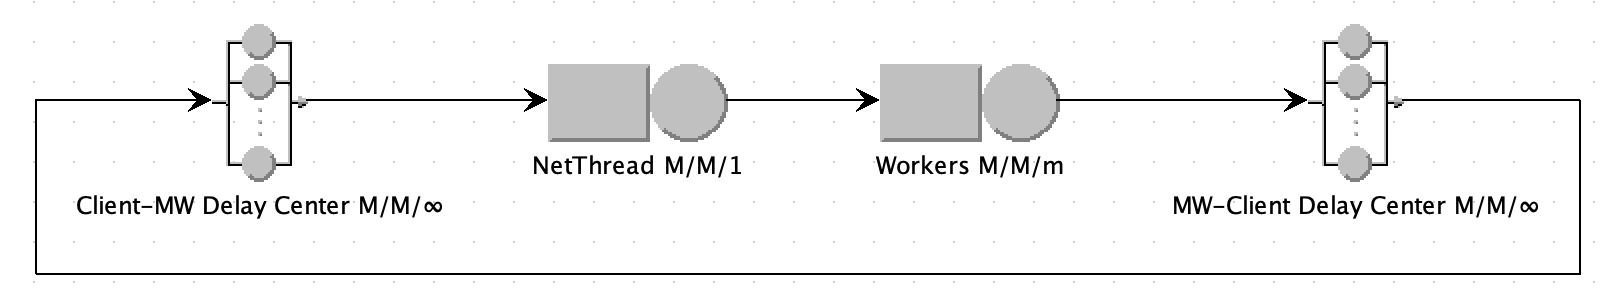
\includegraphics[width=0.9\textwidth]{img/7_qn_1mw.png}
\captionsetup{justification=centering}
\caption{\label{fig:qn_1mw}Queuing Network for One Middleware}
\end{figure}

\begin{table}[!ht]
\resizebox{\linewidth}{!}{%
\begin{tabular}{l|lllllll|lllllll}
\hline
\multirow{2}{*}{Device} & \multicolumn{7}{c|}{Readonly (8 workers/12 clients)} & \multicolumn{7}{c}{Writeonly (64 workers/144 clients)} \\ \cline{2-15} 
                        & $m_i$     & $S_i$    & $\mu_i$   & $V_i$   & $U_i$   & $X_i$   & $R_i$   & $m_i$     & $S_i$     & $\mu_i$     & $V_i$     & $U_i$     & $X_i$    & $R_i$    \\ \hline
Client-MW               & $\infty$    & 0.67     & 0.67       & 1    & -       & -         & 0.67    & $\infty$ & 0.57    & 0.57        & 1     & -     & -        & 0.57   \\
NetThread               & 1         & 0.03     & 0.03       & 1    & 9.46    & 3160.43     & 0.03    & 1        & 0.05    & 0.05        & 1     & 78.66 & 15529.01 & 0.23  \\
Workers                 & 8         & 2.24     & 17.92      & 1    & 89.46   & 3155.11      & 2.41    & 64       & 4.08    & 260.91      & 1     & 100   & 15700.87 & 7.80    \\
MW-Client               & $\infty$    & 0.67     & 0.67       & 1    & -       & -          & 0.66   & $\infty$ & 0.57    & 0.57        & 1     & -     & -        &  0.57  \\ \hline
\end{tabular}
}
\caption{\label{tab:qn_1mw}Network of Queues for One Middleware}
\end{table}

For readonly workload, the system throughput prediction is 3167.67 ops/sec, and response time prediction 3.79 ms, with the measured values 2903.11 ops/sec and 4.07 ms. The utilization of worker threads is as high as 89.46\%, indicating that the workers are about saturated, which is exactly the case, as from Section 3.1 we know the bottleneck is on the bandwidth of the memcached server, and in this model the server has been absorbed into the workers M/M/m queue. The predictions match the realities closely, but the reported throughput is still a little higher than the measured values, because the model is not aware of the fact that the server's sending bandwidth has limited the maximum throughput.

For writeonly workload, the system throughput and response time is predicted as 15733.99 ops/sec and 9.22 ms, while the measured values are 12023.66 ops/sec and 11.84 ms. This does not match so well, and it is understandable: as we can see from the utilization, network threads are utilized by 78.83\% and workers by 100\%, indicating that the bottleneck is on the middleware worker threads; however, the resources of a middleware machine is limited, and not all worker threads are active at the same time, as we have analysed in Section 3.1; therefore even the full utilization of all worker threads is not able to actually yield a theoretical maximum throughput of 64 workers. But the model is not aware of this, it simply assumes that the processing capacity is directly propotional to the number of workers, thus predicting a higher throughput and lower response time than reality.

Therefore, the model captures the system characteristic fairly well, as we have included most of the important system components in the model. It is also useful in identifying the bottleneck, as the utilization values align well with our findings in Section 3.1. However, it does not take the resource limitations into consideration, resulting in some considerable discrepancy between the prediction and reality.

\subsubsection{Two Middlewares}

Similarly, the network of queue for two middlewares is depicted in Figure~\ref{fig:qn_2mw}. The values of input parameters are chosen as described in the beginning. The result for each component is listed in Table~\ref{tab:qn_2mw}, where the last row represents for the entire system and therefore only cares about system throughput and response time.

\begin{figure}[!ht]
\centering
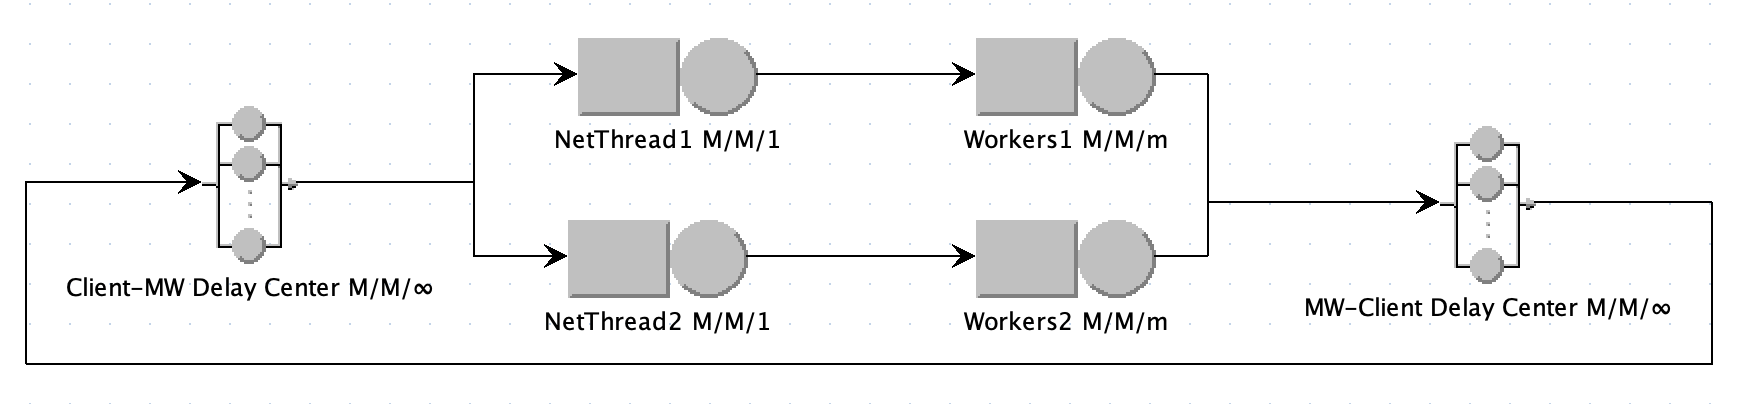
\includegraphics[width=1.0\textwidth]{img/7_qn_2mw.png}
\captionsetup{justification=centering}
\caption{\label{fig:qn_2mw}Network of Queues for Two Middlewares}
\end{figure}

\begin{table}[!ht]
\resizebox{\linewidth}{!}{%
\begin{tabular}{l|lllllll|lllllll}
\hline
\multirow{2}{*}{Device} & \multicolumn{7}{c|}{Readonly (8 workers/12 clients)} & \multicolumn{7}{c}{Writeonly (64 workers/144 clients)} \\ \cline{2-15} 
              & $m_i$     & $S_i$    & $\mu_i$   & $V_i$   & $U_i$   & $X_i$   & $R_i$   & $m_i$     & $S_i$     & $\mu_i$     & $V_i$     & $U_i$     & $X_i$    & $R_i$    \\ \hline
Client-MW     & $\infty$    & 0.61     & 0.61     & 1      & -       & 2910.86 & 0.62    & $\infty$  & 0.58      & 0.58        & 1         & -         & 15503.87 & 0.57   \\
NetThread1    & 1           & 0.03     & 0.03     & 0.5    & 4.44    & 1458.88 & 0.03    & 1         & 0.03      & 0.03        & 0.5       & 23.01     &  7664.37 & 0.39  \\
NetThread2    & 1           & 0.03     & 0.03     & 0.5    & 4.35    & 1469.5  & 0.03    & 1         & 0.03      & 0.03        & 0.5       & 23.18     &  7654.36 & 0.39  \\
Workers1      & 8           & 2.85     & 22.80    & 0.5    & 51.24   & 1453.43 & 2.83    & 64        & 7.85      & 520.40      & 0.5       & 95.16     &  7797.62 & 8.21    \\
Workers2      & 8           & 2.85     & 22.80    & 0.5    & 52.24   & 1470.11 & 2.90    & 64        & 7.85      & 520.40      & 0.5       & 94.83     &  7665.26 & 8.19    \\
MW-Client     & $\infty$    & 0.61     & 0.61     & 1      & -       & 2907.74  & 0.61   & $\infty$   & 0.58      & 0.58        & 1         & -         & 15499.25 & 0.58  \\
System        & -         & -        & -        & -      & -       & 2907.74 & 4.13   & -  & -      & -        & -         & -         & 15499.25 & 9.35  \\

\hline
\end{tabular}
}
\caption{\label{tab:qn_2mw}Results of Network of Queues for Two Middlewares}
\end{table}

As comparison, the measured throughput and response time is 14524.03 ops/sec and 9.81 ms for write-only workload, or 2908.67 ops/sec and 4.07 ms for read-only workload. We can see that the predictions almost perfectly match the measurements, especially for read-only workload. The component utilization in readonly workload is about 4.4\% for both M/M/1 network threads and about 51\% for both M/M/m workers, showing that the load is equally distributed and the burden on workers from One Middleware has been relieved, and the middleware is still not the bottleneck. The utilization of both worker groups sums up to 100\%, which matches the fact that the bottleneck is from the server bandwidth, which has been absorbed into workers in our model.

For write-only workload, the discrepancy between prediction and reality is also smaller than in the One Middleware model, because the resource scarcity is mitigated with doubled middleware, therefore the disadvantage of the model due to unawareness of the resource limitation is also relieved. The utilization of network threads has decreased greatly to only 23\% compared with One Middleware, but the utilization for workers is still as high as 95\%, because the bottleneck is still the memcached server (as we have found in Section 3.2), and the server has been absorbed into the workers M/M/m queues. 

To conclude, our network of queues is even better to model the two middlewares case than the one middleware case. It is successful to predict the system throughput and response time, and utilization values do align with the real bottlenecks we have found in Section 3.2. The discrepancy for write-only workload is also relieved, because the effect of resource limitation has been mitigated by doubled number of middlewares.